\documentclass[twoside]{book}

% Packages required by doxygen
\usepackage{fixltx2e}
\usepackage{calc}
\usepackage{doxygen}
\usepackage[export]{adjustbox} % also loads graphicx
\usepackage{graphicx}
\usepackage[utf8]{inputenc}
\usepackage{makeidx}
\usepackage{multicol}
\usepackage{multirow}
\PassOptionsToPackage{warn}{textcomp}
\usepackage{textcomp}
\usepackage[nointegrals]{wasysym}
\usepackage[table]{xcolor}

% Font selection
\usepackage[T1]{fontenc}
\usepackage[scaled=.90]{helvet}
\usepackage{courier}
\usepackage{amssymb}
\usepackage{sectsty}
\renewcommand{\familydefault}{\sfdefault}
\allsectionsfont{%
  \fontseries{bc}\selectfont%
  \color{darkgray}%
}
\renewcommand{\DoxyLabelFont}{%
  \fontseries{bc}\selectfont%
  \color{darkgray}%
}
\newcommand{\+}{\discretionary{\mbox{\scriptsize$\hookleftarrow$}}{}{}}

% Page & text layout
\usepackage{geometry}
\geometry{%
  a4paper,%
  top=2.5cm,%
  bottom=2.5cm,%
  left=2.5cm,%
  right=2.5cm%
}
\tolerance=750
\hfuzz=15pt
\hbadness=750
\setlength{\emergencystretch}{15pt}
\setlength{\parindent}{0cm}
\setlength{\parskip}{3ex plus 2ex minus 2ex}
\makeatletter
\renewcommand{\paragraph}{%
  \@startsection{paragraph}{4}{0ex}{-1.0ex}{1.0ex}{%
    \normalfont\normalsize\bfseries\SS@parafont%
  }%
}
\renewcommand{\subparagraph}{%
  \@startsection{subparagraph}{5}{0ex}{-1.0ex}{1.0ex}{%
    \normalfont\normalsize\bfseries\SS@subparafont%
  }%
}
\makeatother

% Headers & footers
\usepackage{fancyhdr}
\pagestyle{fancyplain}
\fancyhead[LE]{\fancyplain{}{\bfseries\thepage}}
\fancyhead[CE]{\fancyplain{}{}}
\fancyhead[RE]{\fancyplain{}{\bfseries\leftmark}}
\fancyhead[LO]{\fancyplain{}{\bfseries\rightmark}}
\fancyhead[CO]{\fancyplain{}{}}
\fancyhead[RO]{\fancyplain{}{\bfseries\thepage}}
\fancyfoot[LE]{\fancyplain{}{}}
\fancyfoot[CE]{\fancyplain{}{}}
\fancyfoot[RE]{\fancyplain{}{\bfseries\scriptsize Generated by Doxygen }}
\fancyfoot[LO]{\fancyplain{}{\bfseries\scriptsize Generated by Doxygen }}
\fancyfoot[CO]{\fancyplain{}{}}
\fancyfoot[RO]{\fancyplain{}{}}
\renewcommand{\footrulewidth}{0.4pt}
\renewcommand{\chaptermark}[1]{%
  \markboth{#1}{}%
}
\renewcommand{\sectionmark}[1]{%
  \markright{\thesection\ #1}%
}

% Indices & bibliography
\usepackage{natbib}
\usepackage[titles]{tocloft}
\setcounter{tocdepth}{3}
\setcounter{secnumdepth}{5}
\makeindex

% Hyperlinks (required, but should be loaded last)
\usepackage{ifpdf}
\ifpdf
  \usepackage[pdftex,pagebackref=true]{hyperref}
\else
  \usepackage[ps2pdf,pagebackref=true]{hyperref}
\fi
\hypersetup{%
  colorlinks=true,%
  linkcolor=blue,%
  citecolor=blue,%
  unicode%
}

% Custom commands
\newcommand{\clearemptydoublepage}{%
  \newpage{\pagestyle{empty}\cleardoublepage}%
}

\usepackage{caption}
\captionsetup{labelsep=space,justification=centering,font={bf},singlelinecheck=off,skip=4pt,position=top}

%===== C O N T E N T S =====

\begin{document}

% Titlepage & ToC
\hypersetup{pageanchor=false,
             bookmarksnumbered=true,
             pdfencoding=unicode
            }
\pagenumbering{roman}
\begin{titlepage}
\vspace*{7cm}
\begin{center}%
{\Large orcs }\\
\vspace*{1cm}
{\large Generated by Doxygen 1.8.11}\\
\end{center}
\end{titlepage}
\clearemptydoublepage
\tableofcontents
\clearemptydoublepage
\pagenumbering{arabic}
\hypersetup{pageanchor=true}

%--- Begin generated contents ---
\chapter{T\+O\+DO}
\label{md__home_djordje_Desktop_orcs_src_todo}
\hypertarget{md__home_djordje_Desktop_orcs_src_todo}{}

\begin{DoxyItemize}
\item \hyperlink{packet_8c}{packet.\+c}
\item \hyperlink{packet_8h}{packet.\+h}
\item implement \hyperlink{color_8h}{color.\+h} better
\end{DoxyItemize}

\subsection*{U\+A\+RT -\/ Motion }


\begin{DoxyItemize}
\item uart\+\_\+transmit\+\_\+bytes
\item uart\+\_\+receieve\+\_\+bytes
\item write python script that parses rx packet on PC
\item test uart\+\_\+transmit\+\_\+packet
\item ask for current position
\item print current position as integer
\item set current position
\item check if command which is sent -\/ process if incomed \textquotesingle{}A\textquotesingle{} character
\item main reorganize
\end{DoxyItemize}

scheduler -\/$>$ task -\/$>$ motion\+\_\+go(x,y,velocity); -\/$>$ motion\+\_\+stop() -\/$>$ motion\+\_\+get\+\_\+status(); //where to put?

motion\+: implement motion\+\_\+go -\/$>$ packet\+\_\+send(type, data) -\/$>$ uart\+\_\+transmit 
\chapter{Class Index}
\section{Class List}
Here are the classes, structs, unions and interfaces with brief descriptions\+:\begin{DoxyCompactList}
\item\contentsline{section}{\hyperlink{structpacket__t}{packet\+\_\+t} }{\pageref{structpacket__t}}{}
\end{DoxyCompactList}

\chapter{File Index}
\section{File List}
Here is a list of all documented files with brief descriptions\+:\begin{DoxyCompactList}
\item\contentsline{section}{/home/djordje/\+Desktop/orcs/src/\hyperlink{color_8c}{color.\+c} \\*Functions for setting the default printf() color }{\pageref{color_8c}}{}
\item\contentsline{section}{/home/djordje/\+Desktop/orcs/src/\hyperlink{color_8h}{color.\+h} \\*Defines all of the A\+N\+SI terminal escape codes that modify the color of text }{\pageref{color_8h}}{}
\item\contentsline{section}{/home/djordje/\+Desktop/orcs/src/\hyperlink{config_8c}{config.\+c} }{\pageref{config_8c}}{}
\item\contentsline{section}{/home/djordje/\+Desktop/orcs/src/\hyperlink{config_8h}{config.\+h} \\*Robot configuration file }{\pageref{config_8h}}{}
\item\contentsline{section}{/home/djordje/\+Desktop/orcs/src/\hyperlink{motion_8c}{motion.\+c} }{\pageref{motion_8c}}{}
\item\contentsline{section}{/home/djordje/\+Desktop/orcs/src/\hyperlink{motion_8h}{motion.\+h} }{\pageref{motion_8h}}{}
\item\contentsline{section}{/home/djordje/\+Desktop/orcs/src/\hyperlink{motioncmd_8h}{motioncmd.\+h} }{\pageref{motioncmd_8h}}{}
\item\contentsline{section}{/home/djordje/\+Desktop/orcs/src/\hyperlink{packet_8c}{packet.\+c} }{\pageref{packet_8c}}{}
\item\contentsline{section}{/home/djordje/\+Desktop/orcs/src/\hyperlink{packet_8h}{packet.\+h} \\*Packet status tracking enumeration ~\newline
}{\pageref{packet_8h}}{}
\item\contentsline{section}{/home/djordje/\+Desktop/orcs/src/\hyperlink{uart_8c}{uart.\+c} \\*Inits uart to baud rate 57600. Functions for uart data manipulation }{\pageref{uart_8c}}{}
\item\contentsline{section}{/home/djordje/\+Desktop/orcs/src/\hyperlink{uart_8h}{uart.\+h} }{\pageref{uart_8h}}{}
\end{DoxyCompactList}

\chapter{Class Documentation}
\hypertarget{structpacket__t}{}\section{packet\+\_\+t Struct Reference}
\label{structpacket__t}\index{packet\+\_\+t@{packet\+\_\+t}}


{\ttfamily \#include $<$packet.\+h$>$}

\subsection*{Public Attributes}
\begin{DoxyCompactItemize}
\item 
uint8\+\_\+t {\bfseries sync}\hypertarget{structpacket__t_a76553624e98cd50b114d0784abf2c7d5}{}\label{structpacket__t_a76553624e98cd50b114d0784abf2c7d5}

\item 
uint8\+\_\+t {\bfseries crc}\hypertarget{structpacket__t_a2d535881aafa6b7fe4bb93b6bf69989b}{}\label{structpacket__t_a2d535881aafa6b7fe4bb93b6bf69989b}

\item 
uint8\+\_\+t {\bfseries type}\hypertarget{structpacket__t_afa6fef69d5697c4e07fc8e582e2d578b}{}\label{structpacket__t_afa6fef69d5697c4e07fc8e582e2d578b}

\item 
uint8\+\_\+t {\bfseries size}\hypertarget{structpacket__t_accc302955ca1bc6f75c387b25001208e}{}\label{structpacket__t_accc302955ca1bc6f75c387b25001208e}

\item 
uint8\+\_\+t {\bfseries data} \mbox{[}M\+A\+X\+\_\+\+P\+K\+T\+\_\+\+S\+I\+ZE-\/P\+A\+C\+K\+E\+T\+\_\+\+H\+E\+A\+D\+ER\mbox{]}\hypertarget{structpacket__t_ad772e0b13e249e30cb343a9ffb769389}{}\label{structpacket__t_ad772e0b13e249e30cb343a9ffb769389}

\item 
uint8\+\_\+t {\bfseries packet\+\_\+ptr}\hypertarget{structpacket__t_a91a22b40a5047bfb9e02aa77b75a4279}{}\label{structpacket__t_a91a22b40a5047bfb9e02aa77b75a4279}

\item 
enum Packet\+Status {\bfseries status}\hypertarget{structpacket__t_a25fc56c4d2c72868ab500729ccfdc316}{}\label{structpacket__t_a25fc56c4d2c72868ab500729ccfdc316}

\end{DoxyCompactItemize}


\subsection{Detailed Description}
Motion U\+A\+RT packet S\+C\+T\+Lxxxxxxxx

S -\/ 1 Byte sync (0x3c) ~\newline
 C -\/ 1 Byte checksum ( upper nibble -\/ header checksum, lower~\newline
 nibble payload checksum ) ~\newline
 T -\/ 1 Byte type ~\newline
 L -\/ 1 Byte payload length ~\newline
 x -\/ L Bytes data 

The documentation for this struct was generated from the following file\+:\begin{DoxyCompactItemize}
\item 
/home/djordje/\+Desktop/orcs/src/\hyperlink{packet_8h}{packet.\+h}\end{DoxyCompactItemize}

\chapter{File Documentation}
\hypertarget{color_8h}{}\section{/home/djordje/\+Desktop/orcs/src/color.h File Reference}
\label{color_8h}\index{/home/djordje/\+Desktop/orcs/src/color.\+h@{/home/djordje/\+Desktop/orcs/src/color.\+h}}


Defines all of the A\+N\+SI terminal escape codes that modify the color of text.  


This graph shows which files directly or indirectly include this file\+:\nopagebreak
\begin{figure}[H]
\begin{center}
\leavevmode
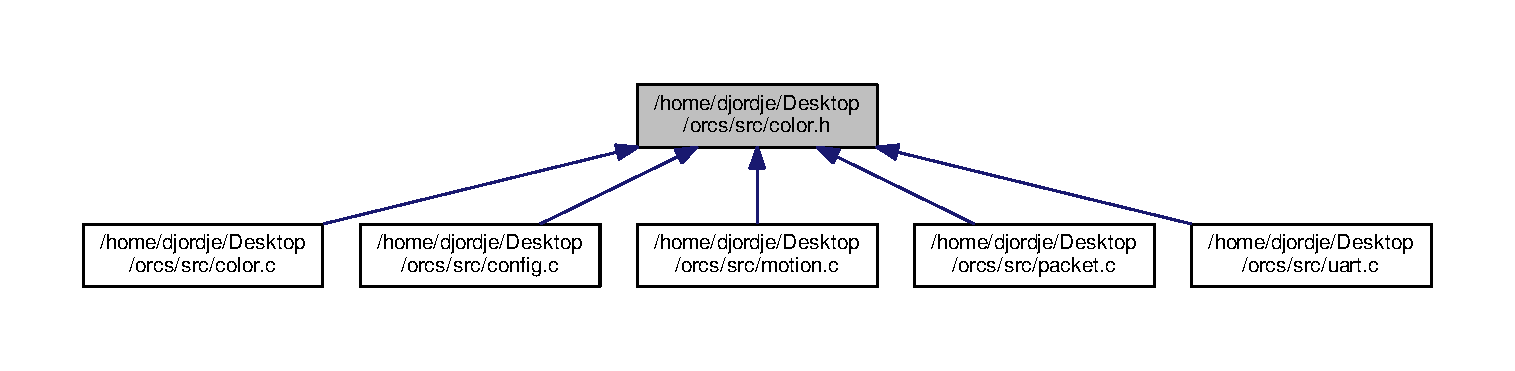
\includegraphics[width=350pt]{color_8h__dep__incl}
\end{center}
\end{figure}
\subsection*{Macros}
\begin{DoxyCompactItemize}
\item 
\#define {\bfseries B\+L\+A\+C\+K\+\_\+\+T\+E\+XT}~\char`\"{}\textbackslash{}033\mbox{[}30;1m\char`\"{}\hypertarget{color_8h_aa8716c5a8fe75c169f85f841cf886e2d}{}\label{color_8h_aa8716c5a8fe75c169f85f841cf886e2d}

\item 
\#define {\bfseries R\+E\+D\+\_\+\+T\+E\+XT}~\char`\"{}\textbackslash{}033\mbox{[}31;1m\char`\"{}\hypertarget{color_8h_ac6b49286f191080eef7f1891a32b6596}{}\label{color_8h_ac6b49286f191080eef7f1891a32b6596}

\item 
\#define {\bfseries G\+R\+E\+E\+N\+\_\+\+T\+E\+XT}~\char`\"{}\textbackslash{}033\mbox{[}32;1m\char`\"{}\hypertarget{color_8h_aaad9cb092d673eb55addd81bdc69f532}{}\label{color_8h_aaad9cb092d673eb55addd81bdc69f532}

\item 
\#define {\bfseries Y\+E\+L\+L\+O\+W\+\_\+\+T\+E\+XT}~\char`\"{}\textbackslash{}033\mbox{[}33;1m\char`\"{}\hypertarget{color_8h_a4b117bf78d42386fd744ff9db8c0e9e5}{}\label{color_8h_a4b117bf78d42386fd744ff9db8c0e9e5}

\item 
\#define {\bfseries B\+L\+U\+E\+\_\+\+T\+E\+XT}~\char`\"{}\textbackslash{}033\mbox{[}34;1m\char`\"{}\hypertarget{color_8h_a523653b137c1298fa4014e26488bee76}{}\label{color_8h_a523653b137c1298fa4014e26488bee76}

\item 
\#define {\bfseries M\+A\+G\+E\+N\+T\+A\+\_\+\+T\+E\+XT}~\char`\"{}\textbackslash{}033\mbox{[}35;1m\char`\"{}\hypertarget{color_8h_ae841e02c40ae502e3e72c0c02c006ff7}{}\label{color_8h_ae841e02c40ae502e3e72c0c02c006ff7}

\item 
\#define {\bfseries C\+Y\+A\+N\+\_\+\+T\+E\+XT}~\char`\"{}\textbackslash{}033\mbox{[}36;1m\char`\"{}\hypertarget{color_8h_aae276f658ffe000aaf9d7dacb15f3009}{}\label{color_8h_aae276f658ffe000aaf9d7dacb15f3009}

\item 
\#define {\bfseries W\+H\+I\+T\+E\+\_\+\+T\+E\+XT}~\char`\"{}\textbackslash{}033\mbox{[}37;1m\char`\"{}\hypertarget{color_8h_aea19743fab227a2e9877bc45c5d52f40}{}\label{color_8h_aea19743fab227a2e9877bc45c5d52f40}

\item 
\#define {\bfseries O\+R\+A\+N\+G\+E\+\_\+\+T\+E\+XT}~\char`\"{}\textbackslash{}033\mbox{[}40;1m\char`\"{}\hypertarget{color_8h_a9ff9d46c0e7ff13b7b6d6267404df407}{}\label{color_8h_a9ff9d46c0e7ff13b7b6d6267404df407}

\item 
\#define {\bfseries B\+O\+L\+D\+\_\+\+B\+L\+A\+C\+K\+\_\+\+T\+E\+XT}~\char`\"{}\textbackslash{}033\mbox{[}1m\textbackslash{}033\mbox{[}30m;1m\char`\"{}\hypertarget{color_8h_a48c5595a94b261f15383ba07f18a5eb6}{}\label{color_8h_a48c5595a94b261f15383ba07f18a5eb6}

\item 
\#define {\bfseries B\+O\+L\+D\+\_\+\+R\+E\+D\+\_\+\+T\+E\+XT}~\char`\"{}\textbackslash{}033\mbox{[}1m\textbackslash{}033\mbox{[}31m;1m\char`\"{}\hypertarget{color_8h_a1de1e321417270f78d26950fbccd560a}{}\label{color_8h_a1de1e321417270f78d26950fbccd560a}

\item 
\#define {\bfseries B\+O\+L\+D\+\_\+\+G\+R\+E\+E\+N\+\_\+\+T\+E\+XT}~\char`\"{}\textbackslash{}033\mbox{[}1m\textbackslash{}033\mbox{[}32m;1m\char`\"{}\hypertarget{color_8h_a4c6b7d748b0f1fe8365e2ce507766812}{}\label{color_8h_a4c6b7d748b0f1fe8365e2ce507766812}

\item 
\#define {\bfseries B\+O\+L\+D\+\_\+\+Y\+E\+L\+L\+O\+W\+\_\+\+T\+E\+XT}~\char`\"{}\textbackslash{}033\mbox{[}1m\textbackslash{}033\mbox{[}33m;1m\char`\"{}\hypertarget{color_8h_a537e6899b5d79ecab537f0d5ffe1089e}{}\label{color_8h_a537e6899b5d79ecab537f0d5ffe1089e}

\item 
\#define {\bfseries B\+O\+L\+D\+\_\+\+B\+L\+U\+E\+\_\+\+T\+E\+XT}~\char`\"{}\textbackslash{}033\mbox{[}1m\textbackslash{}033\mbox{[}34m;1m\char`\"{}\hypertarget{color_8h_a363d994e40d33a58f24dc36eaaac5c44}{}\label{color_8h_a363d994e40d33a58f24dc36eaaac5c44}

\item 
\#define {\bfseries B\+O\+L\+D\+\_\+\+M\+A\+G\+E\+N\+T\+A\+\_\+\+T\+E\+XT}~\char`\"{}\textbackslash{}033\mbox{[}1m\textbackslash{}033\mbox{[}35m;1m\char`\"{}\hypertarget{color_8h_a98867c2616d4ae08be143f019d6365f2}{}\label{color_8h_a98867c2616d4ae08be143f019d6365f2}

\item 
\#define {\bfseries B\+O\+L\+D\+\_\+\+C\+Y\+A\+N\+\_\+\+T\+E\+XT}~\char`\"{}\textbackslash{}033\mbox{[}1m\textbackslash{}033\mbox{[}36m;1m\char`\"{}\hypertarget{color_8h_af375e4529e05c4c6d986326254313e3f}{}\label{color_8h_af375e4529e05c4c6d986326254313e3f}

\item 
\#define {\bfseries B\+O\+L\+D\+\_\+\+W\+H\+I\+T\+E\+\_\+\+T\+E\+XT}~\char`\"{}\textbackslash{}033\mbox{[}1m\textbackslash{}033\mbox{[}37m;1m\char`\"{}\hypertarget{color_8h_a4211e6b437766aa2f5e07e52e7a7b739}{}\label{color_8h_a4211e6b437766aa2f5e07e52e7a7b739}

\end{DoxyCompactItemize}
\subsection*{Functions}
\begin{DoxyCompactItemize}
\item 
void {\bfseries print\+\_\+red} (void)\hypertarget{color_8h_a56e707b248168b71cd3ca77f0a24422e}{}\label{color_8h_a56e707b248168b71cd3ca77f0a24422e}

\item 
void {\bfseries print\+\_\+yellow} (void)\hypertarget{color_8h_a197267070fe71d5836349da951f38961}{}\label{color_8h_a197267070fe71d5836349da951f38961}

\item 
void {\bfseries print\+\_\+blue} (void)\hypertarget{color_8h_a757c47197a51d1e67b43d1afae5c7c9f}{}\label{color_8h_a757c47197a51d1e67b43d1afae5c7c9f}

\item 
void {\bfseries print\+\_\+green} (void)\hypertarget{color_8h_a983ca8a8ba6530d8de25633e0944ef35}{}\label{color_8h_a983ca8a8ba6530d8de25633e0944ef35}

\item 
void {\bfseries print\+\_\+orange} (void)\hypertarget{color_8h_a2feabd20c70965f5fbe3af82c82d14e9}{}\label{color_8h_a2feabd20c70965f5fbe3af82c82d14e9}

\item 
void {\bfseries print\+\_\+cyan} (void)\hypertarget{color_8h_a83dad9942463b885f9187935e78ba676}{}\label{color_8h_a83dad9942463b885f9187935e78ba676}

\item 
void {\bfseries print\+\_\+reset} (void)\hypertarget{color_8h_aa4f6858ed3ecdad5501013ac4001c9ca}{}\label{color_8h_aa4f6858ed3ecdad5501013ac4001c9ca}

\end{DoxyCompactItemize}


\subsection{Detailed Description}
Defines all of the A\+N\+SI terminal escape codes that modify the color of text. 


\hypertarget{packet_8h}{}\section{/home/djordje/\+Desktop/orcs/src/packet.h File Reference}
\label{packet_8h}\index{/home/djordje/\+Desktop/orcs/src/packet.\+h@{/home/djordje/\+Desktop/orcs/src/packet.\+h}}


Packet status tracking enumeration ~\newline
.  


{\ttfamily \#include $<$stdint.\+h$>$}\\*
Include dependency graph for packet.\+h\+:\nopagebreak
\begin{figure}[H]
\begin{center}
\leavevmode
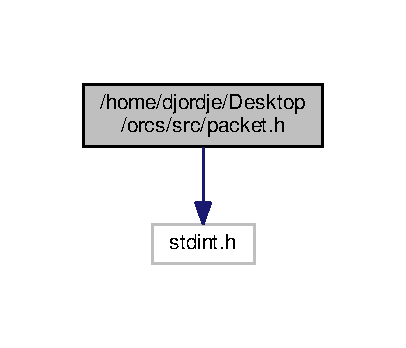
\includegraphics[width=195pt]{packet_8h__incl}
\end{center}
\end{figure}
This graph shows which files directly or indirectly include this file\+:\nopagebreak
\begin{figure}[H]
\begin{center}
\leavevmode
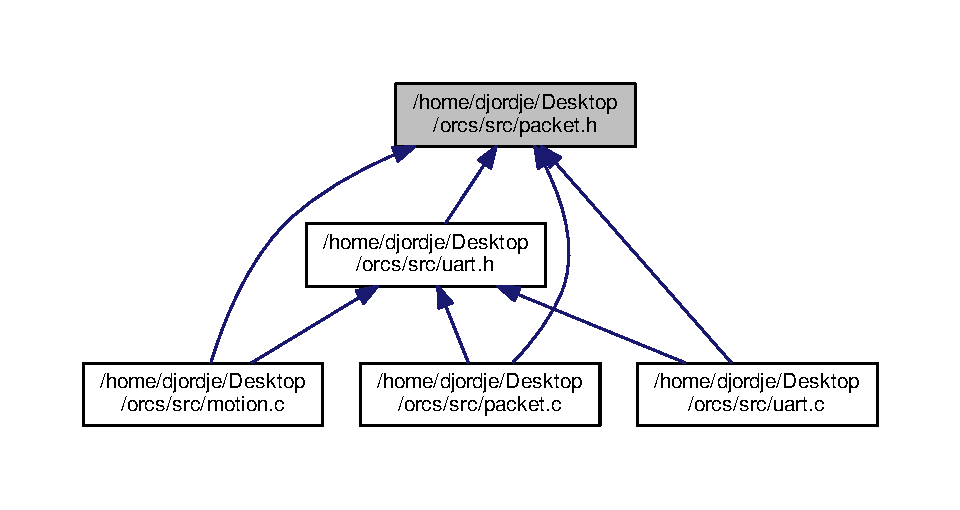
\includegraphics[width=350pt]{packet_8h__dep__incl}
\end{center}
\end{figure}
\subsection*{Classes}
\begin{DoxyCompactItemize}
\item 
struct \hyperlink{structt__packet}{t\+\_\+packet}
\end{DoxyCompactItemize}
\subsection*{Macros}
\begin{DoxyCompactItemize}
\item 
\#define {\bfseries M\+A\+X\+\_\+\+P\+K\+T\+\_\+\+S\+I\+ZE}~32\hypertarget{packet_8h_aa173f20e15ba9658bf440a973ef6d8ca}{}\label{packet_8h_aa173f20e15ba9658bf440a973ef6d8ca}

\item 
\#define {\bfseries P\+A\+C\+K\+E\+T\+\_\+\+H\+E\+A\+D\+ER}~4\hypertarget{packet_8h_a1aa8b6627486da5c445e6bdbe5c2ed0b}{}\label{packet_8h_a1aa8b6627486da5c445e6bdbe5c2ed0b}

\item 
\#define {\bfseries M\+A\+X\+\_\+\+T\+X\+\_\+\+P\+A\+C\+K\+E\+TS}~10\hypertarget{packet_8h_a6925c0c2ae42b3db5dceb74921d307b5}{}\label{packet_8h_a6925c0c2ae42b3db5dceb74921d307b5}

\item 
\#define {\bfseries P\+A\+C\+K\+E\+T\+\_\+\+S\+Y\+NC}~0x3c\hypertarget{packet_8h_a97f8bd380af390f6660657b1711c95f4}{}\label{packet_8h_a97f8bd380af390f6660657b1711c95f4}

\end{DoxyCompactItemize}
\subsection*{Typedefs}
\begin{DoxyCompactItemize}
\item 
typedef struct \hyperlink{structt__packet}{t\+\_\+packet} \hyperlink{packet_8h_a452e8232d6f43e3b74f168306a406f9d}{t\+\_\+packet}
\end{DoxyCompactItemize}
\subsection*{Enumerations}
\begin{DoxyCompactItemize}
\item 
enum {\bfseries Packet\+Status} \{ \\*
{\bfseries free\+\_\+to\+\_\+use}, 
{\bfseries writing\+\_\+packet}, 
{\bfseries ready\+\_\+to\+\_\+send}, 
{\bfseries sending}, 
\\*
{\bfseries free\+\_\+to\+\_\+verify}
 \}\hypertarget{packet_8h_a4bfd4d15be352a21c38bec38fc710d46}{}\label{packet_8h_a4bfd4d15be352a21c38bec38fc710d46}

\end{DoxyCompactItemize}
\subsection*{Functions}
\begin{DoxyCompactItemize}
\item 
void \hyperlink{packet_8h_a1cfcb289613567532e25ec91dff35b7c}{uart\+\_\+pkt\+\_\+en} (uint8\+\_\+t uen)
\item 
\hyperlink{structt__packet}{t\+\_\+packet} $\ast$ \hyperlink{packet_8h_adc7fcb126526a7a03af49d6ea6d4c57c}{try\+\_\+read\+\_\+packet} (void)
\item 
void \hyperlink{packet_8h_acaa8e038792934459fe02b0d38a08484}{tx\+\_\+packets\+\_\+init} (void)
\item 
\hyperlink{structt__packet}{t\+\_\+packet} $\ast$ \hyperlink{packet_8h_a6a5655d1feb2632f9ed82d02a3d1f2a4}{find\+\_\+free\+\_\+packet} (void)
\item 
void \hyperlink{packet_8h_a50271e9b68516a6b862d2964237e189b}{packet\+\_\+prepare} (uint8\+\_\+t type)
\item 
void \hyperlink{packet_8h_acaf4a4e2fbb83aacc9e2ed4f29adc172}{packet\+\_\+put\+\_\+byte} (int8\+\_\+t byte)
\item 
void \hyperlink{packet_8h_a3650e9141d3b4c50372773d750f69fd5}{packet\+\_\+put\+\_\+word} (int16\+\_\+t word)
\item 
void \hyperlink{packet_8h_abdd3690e3729c72dda55bbfa4ace9689}{packet\+\_\+end} (void)
\item 
void \hyperlink{packet_8h_a32aa640412282bba65c1a2d6358bdf2e}{packet\+\_\+verify} (\hyperlink{structt__packet}{t\+\_\+packet} $\ast$packet)
\item 
\hyperlink{structt__packet}{t\+\_\+packet} $\ast$ {\bfseries get\+\_\+selected\+\_\+tx\+\_\+packet} (uint8\+\_\+t select)\hypertarget{packet_8h_acf730aa9517c14513d54d8acbd278d44}{}\label{packet_8h_acf730aa9517c14513d54d8acbd278d44}

\item 
void \hyperlink{packet_8h_a549436969a91be94e35a0c1701384695}{print\+\_\+packet} (\hyperlink{structt__packet}{t\+\_\+packet} $\ast$packet)
\item 
void \hyperlink{packet_8h_ab43a99e9be563e7e6e4ac4b79970b389}{print\+\_\+rx\+\_\+packet} (\hyperlink{structt__packet}{t\+\_\+packet} $\ast$packet)
\end{DoxyCompactItemize}


\subsection{Detailed Description}
Packet status tracking enumeration ~\newline
. 

\begin{DoxyRefDesc}{Todo}
\item[\hyperlink{todo__todo000005}{Todo}]pacet is free when verification is over Packet structure ~\newline
Functions for manipulation with packets \end{DoxyRefDesc}


\subsection{Typedef Documentation}
\index{packet.\+h@{packet.\+h}!t\+\_\+packet@{t\+\_\+packet}}
\index{t\+\_\+packet@{t\+\_\+packet}!packet.\+h@{packet.\+h}}
\subsubsection[{\texorpdfstring{t\+\_\+packet}{t_packet}}]{\setlength{\rightskip}{0pt plus 5cm}typedef struct {\bf t\+\_\+packet} {\bf t\+\_\+packet}}\hypertarget{packet_8h_a452e8232d6f43e3b74f168306a406f9d}{}\label{packet_8h_a452e8232d6f43e3b74f168306a406f9d}
Motion U\+A\+RT packet S\+C\+T\+Lxxxxxxxx

S -\/ 1 Byte sync (0x3c) ~\newline
 C -\/ 1 Byte checksum ( upper nibble -\/ header checksum, lower~\newline
 nibble payload checksum ) ~\newline
 T -\/ 1 Byte type ~\newline
 L -\/ 1 Byte payload length ~\newline
 x -\/ L Bytes data 

\subsection{Function Documentation}
\index{packet.\+h@{packet.\+h}!find\+\_\+free\+\_\+packet@{find\+\_\+free\+\_\+packet}}
\index{find\+\_\+free\+\_\+packet@{find\+\_\+free\+\_\+packet}!packet.\+h@{packet.\+h}}
\subsubsection[{\texorpdfstring{find\+\_\+free\+\_\+packet(void)}{find_free_packet(void)}}]{\setlength{\rightskip}{0pt plus 5cm}{\bf t\+\_\+packet}$\ast$ find\+\_\+free\+\_\+packet (
\begin{DoxyParamCaption}
\item[{void}]{}
\end{DoxyParamCaption}
)}\hypertarget{packet_8h_a6a5655d1feb2632f9ed82d02a3d1f2a4}{}\label{packet_8h_a6a5655d1feb2632f9ed82d02a3d1f2a4}
Looks for free packet \begin{DoxyReturn}{Returns}
free packet adress 
\end{DoxyReturn}
\index{packet.\+h@{packet.\+h}!packet\+\_\+end@{packet\+\_\+end}}
\index{packet\+\_\+end@{packet\+\_\+end}!packet.\+h@{packet.\+h}}
\subsubsection[{\texorpdfstring{packet\+\_\+end(void)}{packet_end(void)}}]{\setlength{\rightskip}{0pt plus 5cm}void packet\+\_\+end (
\begin{DoxyParamCaption}
\item[{void}]{}
\end{DoxyParamCaption}
)}\hypertarget{packet_8h_abdd3690e3729c72dda55bbfa4ace9689}{}\label{packet_8h_abdd3690e3729c72dda55bbfa4ace9689}
Ends packet with sync byte and checksum byte ~\newline
Sends packet via U\+A\+RT ~\newline
At the end, changes packet status to \char`\"{}free\+\_\+to\+\_\+use\char`\"{} \index{packet.\+h@{packet.\+h}!packet\+\_\+prepare@{packet\+\_\+prepare}}
\index{packet\+\_\+prepare@{packet\+\_\+prepare}!packet.\+h@{packet.\+h}}
\subsubsection[{\texorpdfstring{packet\+\_\+prepare(uint8\+\_\+t type)}{packet_prepare(uint8_t type)}}]{\setlength{\rightskip}{0pt plus 5cm}void packet\+\_\+prepare (
\begin{DoxyParamCaption}
\item[{uint8\+\_\+t}]{type}
\end{DoxyParamCaption}
)}\hypertarget{packet_8h_a50271e9b68516a6b862d2964237e189b}{}\label{packet_8h_a50271e9b68516a6b862d2964237e189b}
Prepares everything except message data 
\begin{DoxyParams}{Parameters}
{\em type} & -\/ type of command (defined in \hyperlink{motioncmd_8h}{motioncmd.\+h}) \\
\hline
\end{DoxyParams}
\index{packet.\+h@{packet.\+h}!packet\+\_\+put\+\_\+byte@{packet\+\_\+put\+\_\+byte}}
\index{packet\+\_\+put\+\_\+byte@{packet\+\_\+put\+\_\+byte}!packet.\+h@{packet.\+h}}
\subsubsection[{\texorpdfstring{packet\+\_\+put\+\_\+byte(int8\+\_\+t byte)}{packet_put_byte(int8_t byte)}}]{\setlength{\rightskip}{0pt plus 5cm}void packet\+\_\+put\+\_\+byte (
\begin{DoxyParamCaption}
\item[{int8\+\_\+t}]{byte}
\end{DoxyParamCaption}
)}\hypertarget{packet_8h_acaf4a4e2fbb83aacc9e2ed4f29adc172}{}\label{packet_8h_acaf4a4e2fbb83aacc9e2ed4f29adc172}
Puts byte in data array of message packet 
\begin{DoxyParams}{Parameters}
{\em byte} & -\/ byte which needs to put in \\
\hline
\end{DoxyParams}
\index{packet.\+h@{packet.\+h}!packet\+\_\+put\+\_\+word@{packet\+\_\+put\+\_\+word}}
\index{packet\+\_\+put\+\_\+word@{packet\+\_\+put\+\_\+word}!packet.\+h@{packet.\+h}}
\subsubsection[{\texorpdfstring{packet\+\_\+put\+\_\+word(int16\+\_\+t word)}{packet_put_word(int16_t word)}}]{\setlength{\rightskip}{0pt plus 5cm}void packet\+\_\+put\+\_\+word (
\begin{DoxyParamCaption}
\item[{int16\+\_\+t}]{word}
\end{DoxyParamCaption}
)}\hypertarget{packet_8h_a3650e9141d3b4c50372773d750f69fd5}{}\label{packet_8h_a3650e9141d3b4c50372773d750f69fd5}
Puts word in data array of message packet 
\begin{DoxyParams}{Parameters}
{\em word} & -\/ two bytes which need to put in \\
\hline
\end{DoxyParams}
\index{packet.\+h@{packet.\+h}!packet\+\_\+verify@{packet\+\_\+verify}}
\index{packet\+\_\+verify@{packet\+\_\+verify}!packet.\+h@{packet.\+h}}
\subsubsection[{\texorpdfstring{packet\+\_\+verify(t\+\_\+packet $\ast$packet)}{packet_verify(t_packet *packet)}}]{\setlength{\rightskip}{0pt plus 5cm}void packet\+\_\+verify (
\begin{DoxyParamCaption}
\item[{{\bf t\+\_\+packet} $\ast$}]{packet}
\end{DoxyParamCaption}
)}\hypertarget{packet_8h_a32aa640412282bba65c1a2d6358bdf2e}{}\label{packet_8h_a32aa640412282bba65c1a2d6358bdf2e}
Verifies if acknowledge (command \textquotesingle{}A\textquotesingle{}) packet has the same command in data byte as first unverified packet If verification was success, tx\+\_\+packet status changes to \char`\"{}free\+\_\+to\+\_\+use\char`\"{} Otherwise sends that packet again 
\begin{DoxyParams}{Parameters}
{\em packet} & -\/ packet which is received \\
\hline
\end{DoxyParams}
\index{packet.\+h@{packet.\+h}!print\+\_\+packet@{print\+\_\+packet}}
\index{print\+\_\+packet@{print\+\_\+packet}!packet.\+h@{packet.\+h}}
\subsubsection[{\texorpdfstring{print\+\_\+packet(t\+\_\+packet $\ast$packet)}{print_packet(t_packet *packet)}}]{\setlength{\rightskip}{0pt plus 5cm}void print\+\_\+packet (
\begin{DoxyParamCaption}
\item[{{\bf t\+\_\+packet} $\ast$}]{packet}
\end{DoxyParamCaption}
)}\hypertarget{packet_8h_a549436969a91be94e35a0c1701384695}{}\label{packet_8h_a549436969a91be94e35a0c1701384695}
Function made for easier debugging 
\begin{DoxyParams}{Parameters}
{\em packet} & -\/ adress of TX packet which needs to be printed \\
\hline
\end{DoxyParams}
\index{packet.\+h@{packet.\+h}!print\+\_\+rx\+\_\+packet@{print\+\_\+rx\+\_\+packet}}
\index{print\+\_\+rx\+\_\+packet@{print\+\_\+rx\+\_\+packet}!packet.\+h@{packet.\+h}}
\subsubsection[{\texorpdfstring{print\+\_\+rx\+\_\+packet(t\+\_\+packet $\ast$packet)}{print_rx_packet(t_packet *packet)}}]{\setlength{\rightskip}{0pt plus 5cm}void print\+\_\+rx\+\_\+packet (
\begin{DoxyParamCaption}
\item[{{\bf t\+\_\+packet} $\ast$}]{packet}
\end{DoxyParamCaption}
)}\hypertarget{packet_8h_ab43a99e9be563e7e6e4ac4b79970b389}{}\label{packet_8h_ab43a99e9be563e7e6e4ac4b79970b389}
Function made for easier debugging 
\begin{DoxyParams}{Parameters}
{\em packet} & -\/ adress of RX packet to be printed \\
\hline
\end{DoxyParams}
\index{packet.\+h@{packet.\+h}!try\+\_\+read\+\_\+packet@{try\+\_\+read\+\_\+packet}}
\index{try\+\_\+read\+\_\+packet@{try\+\_\+read\+\_\+packet}!packet.\+h@{packet.\+h}}
\subsubsection[{\texorpdfstring{try\+\_\+read\+\_\+packet(void)}{try_read_packet(void)}}]{\setlength{\rightskip}{0pt plus 5cm}{\bf t\+\_\+packet}$\ast$ try\+\_\+read\+\_\+packet (
\begin{DoxyParamCaption}
\item[{void}]{}
\end{DoxyParamCaption}
)}\hypertarget{packet_8h_adc7fcb126526a7a03af49d6ea6d4c57c}{}\label{packet_8h_adc7fcb126526a7a03af49d6ea6d4c57c}
Trys to read data packet \begin{DoxyReturn}{Returns}
packet adress if found, or 0 if packet not found 
\end{DoxyReturn}
\index{packet.\+h@{packet.\+h}!tx\+\_\+packets\+\_\+init@{tx\+\_\+packets\+\_\+init}}
\index{tx\+\_\+packets\+\_\+init@{tx\+\_\+packets\+\_\+init}!packet.\+h@{packet.\+h}}
\subsubsection[{\texorpdfstring{tx\+\_\+packets\+\_\+init(void)}{tx_packets_init(void)}}]{\setlength{\rightskip}{0pt plus 5cm}void tx\+\_\+packets\+\_\+init (
\begin{DoxyParamCaption}
\item[{void}]{}
\end{DoxyParamCaption}
)}\hypertarget{packet_8h_acaa8e038792934459fe02b0d38a08484}{}\label{packet_8h_acaa8e038792934459fe02b0d38a08484}
Initialises packet status to \char`\"{}free\+\_\+to\+\_\+use\char`\"{} \index{packet.\+h@{packet.\+h}!uart\+\_\+pkt\+\_\+en@{uart\+\_\+pkt\+\_\+en}}
\index{uart\+\_\+pkt\+\_\+en@{uart\+\_\+pkt\+\_\+en}!packet.\+h@{packet.\+h}}
\subsubsection[{\texorpdfstring{uart\+\_\+pkt\+\_\+en(uint8\+\_\+t uen)}{uart_pkt_en(uint8_t uen)}}]{\setlength{\rightskip}{0pt plus 5cm}void uart\+\_\+pkt\+\_\+en (
\begin{DoxyParamCaption}
\item[{uint8\+\_\+t}]{uen}
\end{DoxyParamCaption}
)}\hypertarget{packet_8h_a1cfcb289613567532e25ec91dff35b7c}{}\label{packet_8h_a1cfcb289613567532e25ec91dff35b7c}
Enables / disables uart using (second option would be C\+AN) and it will be implemented later. 
\begin{DoxyParams}{Parameters}
{\em uen} & 1 -\/ enabled, 0 -\/ disabled \\
\hline
\end{DoxyParams}

%--- End generated contents ---

% Index
\backmatter
\newpage
\phantomsection
\clearemptydoublepage
\addcontentsline{toc}{chapter}{Index}
\printindex

\end{document}
